\documentclass[]{article}
\usepackage{lmodern}
\usepackage{amssymb,amsmath}
\usepackage{ifxetex,ifluatex}
\usepackage{fixltx2e} % provides \textsubscript
\ifnum 0\ifxetex 1\fi\ifluatex 1\fi=0 % if pdftex
  \usepackage[T1]{fontenc}
  \usepackage[utf8]{inputenc}
\else % if luatex or xelatex
  \ifxetex
    \usepackage{mathspec}
  \else
    \usepackage{fontspec}
  \fi
  \defaultfontfeatures{Ligatures=TeX,Scale=MatchLowercase}
\fi
% use upquote if available, for straight quotes in verbatim environments
\IfFileExists{upquote.sty}{\usepackage{upquote}}{}
% use microtype if available
\IfFileExists{microtype.sty}{%
\usepackage{microtype}
\UseMicrotypeSet[protrusion]{basicmath} % disable protrusion for tt fonts
}{}
\usepackage[margin=1in]{geometry}
\usepackage{hyperref}
\hypersetup{unicode=true,
            pdftitle={NRG Example},
            pdfauthor={Kirstin Holsman},
            pdfborder={0 0 0},
            breaklinks=true}
\urlstyle{same}  % don't use monospace font for urls
\usepackage{color}
\usepackage{fancyvrb}
\newcommand{\VerbBar}{|}
\newcommand{\VERB}{\Verb[commandchars=\\\{\}]}
\DefineVerbatimEnvironment{Highlighting}{Verbatim}{commandchars=\\\{\}}
% Add ',fontsize=\small' for more characters per line
\usepackage{framed}
\definecolor{shadecolor}{RGB}{248,248,248}
\newenvironment{Shaded}{\begin{snugshade}}{\end{snugshade}}
\newcommand{\KeywordTok}[1]{\textcolor[rgb]{0.13,0.29,0.53}{\textbf{{#1}}}}
\newcommand{\DataTypeTok}[1]{\textcolor[rgb]{0.13,0.29,0.53}{{#1}}}
\newcommand{\DecValTok}[1]{\textcolor[rgb]{0.00,0.00,0.81}{{#1}}}
\newcommand{\BaseNTok}[1]{\textcolor[rgb]{0.00,0.00,0.81}{{#1}}}
\newcommand{\FloatTok}[1]{\textcolor[rgb]{0.00,0.00,0.81}{{#1}}}
\newcommand{\ConstantTok}[1]{\textcolor[rgb]{0.00,0.00,0.00}{{#1}}}
\newcommand{\CharTok}[1]{\textcolor[rgb]{0.31,0.60,0.02}{{#1}}}
\newcommand{\SpecialCharTok}[1]{\textcolor[rgb]{0.00,0.00,0.00}{{#1}}}
\newcommand{\StringTok}[1]{\textcolor[rgb]{0.31,0.60,0.02}{{#1}}}
\newcommand{\VerbatimStringTok}[1]{\textcolor[rgb]{0.31,0.60,0.02}{{#1}}}
\newcommand{\SpecialStringTok}[1]{\textcolor[rgb]{0.31,0.60,0.02}{{#1}}}
\newcommand{\ImportTok}[1]{{#1}}
\newcommand{\CommentTok}[1]{\textcolor[rgb]{0.56,0.35,0.01}{\textit{{#1}}}}
\newcommand{\DocumentationTok}[1]{\textcolor[rgb]{0.56,0.35,0.01}{\textbf{\textit{{#1}}}}}
\newcommand{\AnnotationTok}[1]{\textcolor[rgb]{0.56,0.35,0.01}{\textbf{\textit{{#1}}}}}
\newcommand{\CommentVarTok}[1]{\textcolor[rgb]{0.56,0.35,0.01}{\textbf{\textit{{#1}}}}}
\newcommand{\OtherTok}[1]{\textcolor[rgb]{0.56,0.35,0.01}{{#1}}}
\newcommand{\FunctionTok}[1]{\textcolor[rgb]{0.00,0.00,0.00}{{#1}}}
\newcommand{\VariableTok}[1]{\textcolor[rgb]{0.00,0.00,0.00}{{#1}}}
\newcommand{\ControlFlowTok}[1]{\textcolor[rgb]{0.13,0.29,0.53}{\textbf{{#1}}}}
\newcommand{\OperatorTok}[1]{\textcolor[rgb]{0.81,0.36,0.00}{\textbf{{#1}}}}
\newcommand{\BuiltInTok}[1]{{#1}}
\newcommand{\ExtensionTok}[1]{{#1}}
\newcommand{\PreprocessorTok}[1]{\textcolor[rgb]{0.56,0.35,0.01}{\textit{{#1}}}}
\newcommand{\AttributeTok}[1]{\textcolor[rgb]{0.77,0.63,0.00}{{#1}}}
\newcommand{\RegionMarkerTok}[1]{{#1}}
\newcommand{\InformationTok}[1]{\textcolor[rgb]{0.56,0.35,0.01}{\textbf{\textit{{#1}}}}}
\newcommand{\WarningTok}[1]{\textcolor[rgb]{0.56,0.35,0.01}{\textbf{\textit{{#1}}}}}
\newcommand{\AlertTok}[1]{\textcolor[rgb]{0.94,0.16,0.16}{{#1}}}
\newcommand{\ErrorTok}[1]{\textcolor[rgb]{0.64,0.00,0.00}{\textbf{{#1}}}}
\newcommand{\NormalTok}[1]{{#1}}
\usepackage{graphicx,grffile}
\makeatletter
\def\maxwidth{\ifdim\Gin@nat@width>\linewidth\linewidth\else\Gin@nat@width\fi}
\def\maxheight{\ifdim\Gin@nat@height>\textheight\textheight\else\Gin@nat@height\fi}
\makeatother
% Scale images if necessary, so that they will not overflow the page
% margins by default, and it is still possible to overwrite the defaults
% using explicit options in \includegraphics[width, height, ...]{}
\setkeys{Gin}{width=\maxwidth,height=\maxheight,keepaspectratio}
\IfFileExists{parskip.sty}{%
\usepackage{parskip}
}{% else
\setlength{\parindent}{0pt}
\setlength{\parskip}{6pt plus 2pt minus 1pt}
}
\setlength{\emergencystretch}{3em}  % prevent overfull lines
\providecommand{\tightlist}{%
  \setlength{\itemsep}{0pt}\setlength{\parskip}{0pt}}
\setcounter{secnumdepth}{0}
% Redefines (sub)paragraphs to behave more like sections
\ifx\paragraph\undefined\else
\let\oldparagraph\paragraph
\renewcommand{\paragraph}[1]{\oldparagraph{#1}\mbox{}}
\fi
\ifx\subparagraph\undefined\else
\let\oldsubparagraph\subparagraph
\renewcommand{\subparagraph}[1]{\oldsubparagraph{#1}\mbox{}}
\fi

%%% Use protect on footnotes to avoid problems with footnotes in titles
\let\rmarkdownfootnote\footnote%
\def\footnote{\protect\rmarkdownfootnote}

%%% Change title format to be more compact
\usepackage{titling}

% Create subtitle command for use in maketitle
\newcommand{\subtitle}[1]{
  \posttitle{
    \begin{center}\large#1\end{center}
    }
}

\setlength{\droptitle}{-2em}
  \title{NRG Example}
  \pretitle{\vspace{\droptitle}\centering\huge}
  \posttitle{\par}
  \author{Kirstin Holsman}
  \preauthor{\centering\large\emph}
  \postauthor{\par}
  \predate{\centering\large\emph}
  \postdate{\par}
  \date{12/13/2017}


\begin{document}
\maketitle

\subsection{Install the package}\label{install-the-package}

\begin{Shaded}
\begin{Highlighting}[]
  \CommentTok{# install.packages("devtools")}
  \CommentTok{#library("devtools")}
  \CommentTok{#devtools::install_github("kholsman/NRG")}
\end{Highlighting}
\end{Shaded}

\begin{center}\rule{0.5\linewidth}{\linethickness}\end{center}

\subsection{Part 1: Set up}\label{part-1-set-up}

\begin{Shaded}
\begin{Highlighting}[]
  \KeywordTok{rm}\NormalTok{(}\DataTypeTok{list=}\KeywordTok{ls}\NormalTok{())}
  \KeywordTok{graphics.off}\NormalTok{()}
  \KeywordTok{setwd}\NormalTok{(}\StringTok{"/Users/kholsman/GitHub/NRG/NRG"}\NormalTok{)}
  \NormalTok{## some data for Halibut}
    \KeywordTok{load}\NormalTok{(}\StringTok{"data/HalibutC.Rdata"}\NormalTok{)}
    \KeywordTok{load}\NormalTok{(}\StringTok{"data/alldat4B.Rdata"}\NormalTok{)}
    \KeywordTok{load}\NormalTok{(}\StringTok{"data/alldatA3.Rdata"}\NormalTok{)}
    \KeywordTok{load}\NormalTok{(}\StringTok{"data/alldat4CD.Rdata"}\NormalTok{)}
    \KeywordTok{source}\NormalTok{(}\StringTok{"R/bioE.R"}\NormalTok{)}
  \CommentTok{# Set up some parms}
    \NormalTok{hal_par<-}\KeywordTok{list}\NormalTok{(}\DataTypeTok{Ceq=}\DecValTok{2}\NormalTok{,}\DataTypeTok{Req=}\DecValTok{1}\NormalTok{,}\DataTypeTok{Weq=}\DecValTok{1}\NormalTok{,}\DataTypeTok{RFR=}\DecValTok{1}\NormalTok{,}\DataTypeTok{Qox=}\DecValTok{13560}\NormalTok{,}\DataTypeTok{CA=}\FloatTok{0.0627}\NormalTok{,}\DataTypeTok{CB=}\NormalTok{-}\FloatTok{0.108}\NormalTok{,}\DataTypeTok{Tco=}\FloatTok{12.9699}\NormalTok{,}
                  \DataTypeTok{Tcm=}\DecValTok{18}\NormalTok{,}\DataTypeTok{QC=}\FloatTok{3.084}\NormalTok{,}\DataTypeTok{RK4=}\FloatTok{0.3729}\NormalTok{,}\DataTypeTok{RK1=}\FloatTok{0.008}\NormalTok{,}\DataTypeTok{Am=}\FloatTok{0.008}\NormalTok{,}\DataTypeTok{Bact=}\FloatTok{0.2215}\NormalTok{,}
                  \DataTypeTok{logsigma=}\NormalTok{-}\FloatTok{9.412}\NormalTok{,}\DataTypeTok{RA=}\FloatTok{0.0016}\NormalTok{,}\DataTypeTok{RB=}\NormalTok{-}\FloatTok{0.1848}\NormalTok{,}\DataTypeTok{QR=}\FloatTok{0.0644}\NormalTok{,}\DataTypeTok{Trl=}\DecValTok{12}\NormalTok{,}\DataTypeTok{Trm=}\OtherTok{NA}\NormalTok{,}
                  \DataTypeTok{Tro=}\FloatTok{0.25}\NormalTok{,}\DataTypeTok{UA=}\FloatTok{0.0332}\NormalTok{,}\DataTypeTok{UA.sigma=}\FloatTok{0.082}\NormalTok{,}\DataTypeTok{FA=}\FloatTok{0.2}\NormalTok{,}\DataTypeTok{SA=}\FloatTok{0.1181}\NormalTok{,}\DataTypeTok{SA.sigma=}\FloatTok{0.2574}\NormalTok{)}
    \NormalTok{PARMS_USE<-hal_par}
    \CommentTok{# P..Halibut    Epipelagic  Halibut  4.80 kJ  +/-   0.7 2011 Mar Bio : Seasonal cycles }
    \CommentTok{# in whole-body proximate composition and energy content of forage fish vary with }
    \CommentTok{# water depth. Johanna J. Vollenweider • Ron A. Heintz •Lawrence Schaufler • Robert Bradshaw}
    \NormalTok{HalibutED<-}\DecValTok{4800}  \CommentTok{# Halibut energy density}
    \NormalTok{EpreyUse<-}\FloatTok{4598.07} \CommentTok{# average across sizes}
    \NormalTok{ebs_data_lowpreyE<-}\KeywordTok{list}\NormalTok{(}\DataTypeTok{W=}\DecValTok{100}\NormalTok{,}\DataTypeTok{TempC=}\KeywordTok{seq}\NormalTok{(}\DecValTok{0}\NormalTok{,}\DecValTok{25}\NormalTok{,.}\DecValTok{1}\NormalTok{),}\DataTypeTok{Eprey=}\DecValTok{3400}\NormalTok{,}\DataTypeTok{Epred=}\NormalTok{HalibutED,}\DataTypeTok{indgst=}\DecValTok{0}\NormalTok{,}\DataTypeTok{diet=}\DecValTok{0}\NormalTok{)  }\CommentTok{#4184}
    \NormalTok{ebs_data_highpreyE<-}\KeywordTok{list}\NormalTok{(}\DataTypeTok{W=}\DecValTok{100}\NormalTok{,}\DataTypeTok{TempC=}\KeywordTok{seq}\NormalTok{(}\DecValTok{0}\NormalTok{,}\DecValTok{25}\NormalTok{,.}\DecValTok{1}\NormalTok{),}\DataTypeTok{Eprey=}\FloatTok{5539.6}\NormalTok{,}\DataTypeTok{Epred=}\NormalTok{HalibutED,}\DataTypeTok{indgst=}\DecValTok{0}\NormalTok{,}\DataTypeTok{diet=}\DecValTok{0}\NormalTok{)  }\CommentTok{#4184}
    \NormalTok{ebs_data<-}\KeywordTok{list}\NormalTok{(}\DataTypeTok{W=}\DecValTok{100}\NormalTok{,}\DataTypeTok{TempC=}\KeywordTok{seq}\NormalTok{(}\DecValTok{0}\NormalTok{,}\DecValTok{25}\NormalTok{,.}\DecValTok{1}\NormalTok{),}\DataTypeTok{Eprey=}\NormalTok{EpreyUse,}\DataTypeTok{Epred=}\NormalTok{HalibutED,}\DataTypeTok{indgst=}\DecValTok{0}\NormalTok{,}\DataTypeTok{diet=}\DecValTok{0}\NormalTok{)}
\end{Highlighting}
\end{Shaded}

\begin{center}\rule{0.5\linewidth}{\linethickness}\end{center}

\subsection{Part 2: Explore main
functions}\label{part-2-explore-main-functions}

\begin{Shaded}
\begin{Highlighting}[]
  \CommentTok{# G = (Cmax*f(Tc)*RFR)-(R*Act+SDA+F+U)}
    
  \CommentTok{# plot the consumption data and f(Tc) functions}
    \NormalTok{c_data<-ebs_data}
    \NormalTok{c_data$fTCmodel<-function(TempC)\{-.}\DecValTok{5}\NormalTok{*TempC\}}
    \NormalTok{ft<-}\KeywordTok{fTC_fun}\NormalTok{(}\DataTypeTok{par=}\NormalTok{PARMS_USE,}\DataTypeTok{data=}\NormalTok{c_data)}
  \CommentTok{# plot the function}
    \NormalTok{ylimm<-}\KeywordTok{list}\NormalTok{();ylimm[[}\DecValTok{1}\NormalTok{]]<-}\KeywordTok{c}\NormalTok{(}\DecValTok{0}\NormalTok{,}\FloatTok{1.2}\NormalTok{)}
    \KeywordTok{plot}\NormalTok{(ebs_data$TempC,ft,}\DataTypeTok{type=}\StringTok{"l"}\NormalTok{,}\DataTypeTok{xlim=}\KeywordTok{c}\NormalTok{(}\DecValTok{0}\NormalTok{,}\DecValTok{18}\NormalTok{), }\DataTypeTok{ylim=}\NormalTok{ylimm[[}\DecValTok{1}\NormalTok{]],}\DataTypeTok{axes=}\OtherTok{FALSE}\NormalTok{,}\DataTypeTok{ylab=}\StringTok{""}\NormalTok{,}\DataTypeTok{xlab=}\StringTok{""}\NormalTok{,}\DataTypeTok{lwd=}\DecValTok{2}\NormalTok{)}
    \KeywordTok{points}\NormalTok{(FTdat,}\DataTypeTok{pch=}\DecValTok{16}\NormalTok{)}
    \KeywordTok{axis}\NormalTok{(}\DecValTok{1}\NormalTok{);}\KeywordTok{axis}\NormalTok{(}\DecValTok{1}\NormalTok{,}\DataTypeTok{at=}\KeywordTok{c}\NormalTok{(-}\DecValTok{10}\NormalTok{,}\DecValTok{40}\NormalTok{))}
    \KeywordTok{axis}\NormalTok{(}\DecValTok{2}\NormalTok{,}\DataTypeTok{las=}\DecValTok{2}\NormalTok{);}\KeywordTok{axis}\NormalTok{(}\DecValTok{2}\NormalTok{,}\DataTypeTok{at=}\KeywordTok{c}\NormalTok{(-}\DecValTok{10}\NormalTok{,}\DecValTok{10}\NormalTok{))}
    \KeywordTok{abline}\NormalTok{(}\DataTypeTok{v=}\NormalTok{PARMS_USE$Tco,}\DataTypeTok{lty=}\DecValTok{3}\NormalTok{)}
    \KeywordTok{abline}\NormalTok{(}\DataTypeTok{v=}\NormalTok{PARMS_USE$Tcm,}\DataTypeTok{lty=}\DecValTok{3}\NormalTok{)}
    \KeywordTok{abline}\NormalTok{(}\DataTypeTok{v=}\NormalTok{PARMS_USE$Qc,}\DataTypeTok{lty=}\DecValTok{3}\NormalTok{)}
    \KeywordTok{text}\NormalTok{(PARMS_USE$Tco}\FloatTok{-.4}\NormalTok{,ylimm[[}\DecValTok{1}\NormalTok{]][}\DecValTok{2}\NormalTok{]*.}\DecValTok{95}\NormalTok{,}\StringTok{"Tco"}\NormalTok{, }\DataTypeTok{srt =}\DecValTok{90}\NormalTok{)}
    \KeywordTok{text}\NormalTok{(PARMS_USE$Tcm}\FloatTok{-.4}\NormalTok{,ylimm[[}\DecValTok{1}\NormalTok{]][}\DecValTok{2}\NormalTok{]*.}\DecValTok{95}\NormalTok{,}\StringTok{"Tcm"}\NormalTok{, }\DataTypeTok{srt =}\DecValTok{90}\NormalTok{)}
    \KeywordTok{text}\NormalTok{(PARMS_USE$Qc}\FloatTok{-.4}\NormalTok{,ylimm[[}\DecValTok{1}\NormalTok{]][}\DecValTok{2}\NormalTok{]*.}\DecValTok{95}\NormalTok{,}\StringTok{"Qc"}\NormalTok{, }\DataTypeTok{srt =}\DecValTok{90}\NormalTok{)}
    \KeywordTok{mtext}\NormalTok{(}\StringTok{"f(T)"}\NormalTok{,}\DecValTok{2}\NormalTok{,}\DataTypeTok{outer=}\OtherTok{FALSE}\NormalTok{,}\DataTypeTok{line=}\FloatTok{2.5}\NormalTok{,}\DataTypeTok{font=}\DecValTok{2}\NormalTok{,}\DataTypeTok{cex=}\DecValTok{1}\NormalTok{)}
    \KeywordTok{text}\NormalTok{(.}\DecValTok{3}\NormalTok{,ylimm[[}\DecValTok{1}\NormalTok{]][}\DecValTok{2}\NormalTok{],}\StringTok{"a)"}\NormalTok{,}\DataTypeTok{font=}\DecValTok{2}\NormalTok{)}
\end{Highlighting}
\end{Shaded}

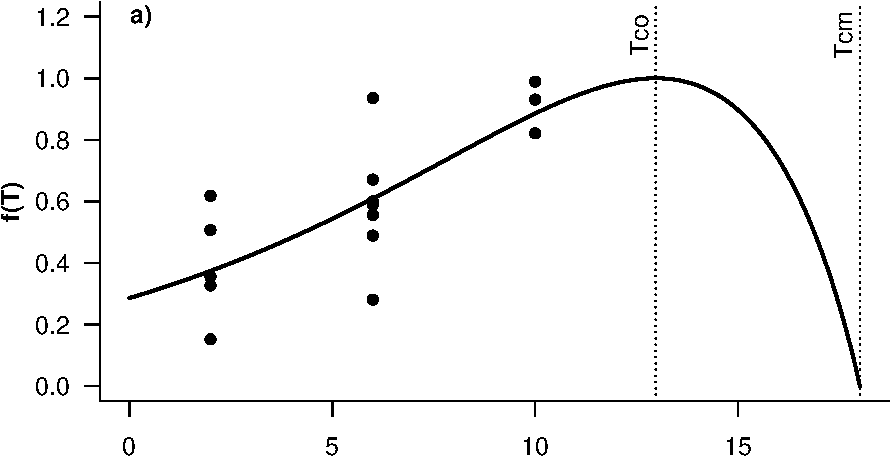
\includegraphics{NRG_summary_files/figure-latex/Part2-1.pdf}

\begin{Shaded}
\begin{Highlighting}[]
  \CommentTok{# now plot swim velocity functions:}
    \NormalTok{vel_dat<-ebs_data}
    \NormalTok{vel_dat$fitLL<-}\OtherTok{FALSE}
    \NormalTok{vel_dat$velobs<-}\OtherTok{NA}
    \NormalTok{veld<-}\KeywordTok{Resp_fun}\NormalTok{(}\DataTypeTok{par=}\NormalTok{PARMS_USE,}\DataTypeTok{data=}\NormalTok{vel_dat)  }\CommentTok{# returns Act, fTr,and Vel}
  
    \KeywordTok{plot}\NormalTok{(ebs_data$TempC,veld$Vel,}\DataTypeTok{type=}\StringTok{"l"}\NormalTok{,}\DataTypeTok{xlim=}\KeywordTok{c}\NormalTok{(}\DecValTok{0}\NormalTok{,}\DecValTok{18}\NormalTok{), }\DataTypeTok{ylim=}\NormalTok{ylimm[[}\DecValTok{1}\NormalTok{]],}\DataTypeTok{axes=}\OtherTok{FALSE}\NormalTok{,}\DataTypeTok{ylab=}\StringTok{""}\NormalTok{,}\DataTypeTok{xlab=}\StringTok{""}\NormalTok{,}\DataTypeTok{lwd=}\DecValTok{2}\NormalTok{,}\DataTypeTok{main=}\StringTok{"Velocity"}\NormalTok{,}\DataTypeTok{line=}\NormalTok{-}\DecValTok{1}\NormalTok{)}
    \KeywordTok{axis}\NormalTok{(}\DecValTok{1}\NormalTok{);}\KeywordTok{axis}\NormalTok{(}\DecValTok{1}\NormalTok{,}\DataTypeTok{at=}\KeywordTok{c}\NormalTok{(-}\DecValTok{10}\NormalTok{,}\DecValTok{40}\NormalTok{));}\KeywordTok{axis}\NormalTok{(}\DecValTok{2}\NormalTok{,}\DataTypeTok{las=}\DecValTok{2}\NormalTok{);}\KeywordTok{axis}\NormalTok{(}\DecValTok{2}\NormalTok{,}\DataTypeTok{at=}\KeywordTok{c}\NormalTok{(-}\DecValTok{10}\NormalTok{,}\DecValTok{10}\NormalTok{))}
    \KeywordTok{abline}\NormalTok{(}\DataTypeTok{v=}\NormalTok{PARMS_USE$Trl,}\DataTypeTok{lty=}\DecValTok{3}\NormalTok{);}\KeywordTok{text}\NormalTok{(PARMS_USE$Trl}\FloatTok{-.4}\NormalTok{,ylimm[[}\DecValTok{1}\NormalTok{]][}\DecValTok{2}\NormalTok{]*.}\DecValTok{8}\NormalTok{,}\StringTok{"Trl"}\NormalTok{, }\DataTypeTok{srt =}\DecValTok{90}\NormalTok{)}
\end{Highlighting}
\end{Shaded}

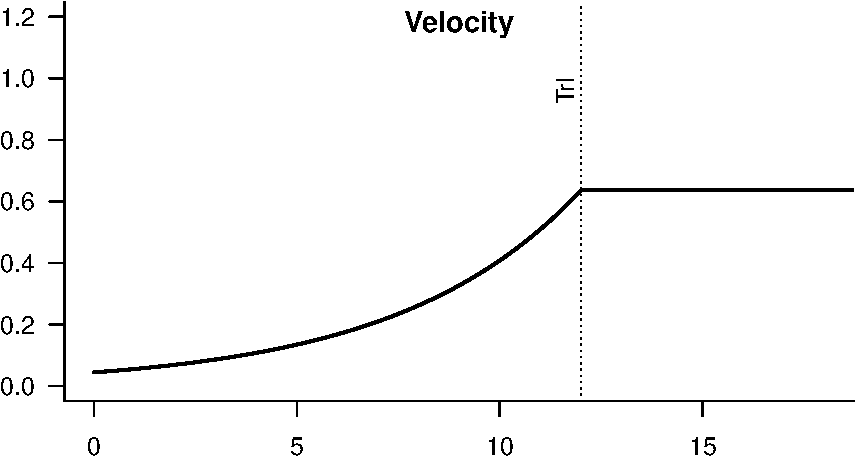
\includegraphics{NRG_summary_files/figure-latex/Part2-2.pdf}

\begin{Shaded}
\begin{Highlighting}[]
    \KeywordTok{plot}\NormalTok{(ebs_data$TempC,veld$Act,}\DataTypeTok{type=}\StringTok{"l"}\NormalTok{,}\DataTypeTok{xlim=}\KeywordTok{c}\NormalTok{(}\DecValTok{0}\NormalTok{,}\DecValTok{18}\NormalTok{), }\DataTypeTok{ylim=}\KeywordTok{c}\NormalTok{(}\DecValTok{0}\NormalTok{,}\DecValTok{2}\NormalTok{),}\DataTypeTok{axes=}\OtherTok{FALSE}\NormalTok{,}\DataTypeTok{ylab=}\StringTok{""}\NormalTok{,}\DataTypeTok{xlab=}\StringTok{""}\NormalTok{,}\DataTypeTok{lwd=}\DecValTok{2}\NormalTok{,}\DataTypeTok{main=}\StringTok{"Activity"}\NormalTok{,}\DataTypeTok{line=}\NormalTok{-}\DecValTok{1}\NormalTok{)}
    \KeywordTok{axis}\NormalTok{(}\DecValTok{1}\NormalTok{);}\KeywordTok{axis}\NormalTok{(}\DecValTok{1}\NormalTok{,}\DataTypeTok{at=}\KeywordTok{c}\NormalTok{(-}\DecValTok{10}\NormalTok{,}\DecValTok{40}\NormalTok{));}\KeywordTok{axis}\NormalTok{(}\DecValTok{2}\NormalTok{,}\DataTypeTok{las=}\DecValTok{2}\NormalTok{);}\KeywordTok{axis}\NormalTok{(}\DecValTok{2}\NormalTok{,}\DataTypeTok{at=}\KeywordTok{c}\NormalTok{(-}\DecValTok{10}\NormalTok{,}\DecValTok{10}\NormalTok{))}
    \KeywordTok{abline}\NormalTok{(}\DataTypeTok{v=}\NormalTok{PARMS_USE$Trl,}\DataTypeTok{lty=}\DecValTok{3}\NormalTok{);}\KeywordTok{text}\NormalTok{(PARMS_USE$Trl}\FloatTok{-.4}\NormalTok{,}\FloatTok{1.5}\NormalTok{,}\StringTok{"Trl"}\NormalTok{, }\DataTypeTok{srt =}\DecValTok{90}\NormalTok{)}
\end{Highlighting}
\end{Shaded}

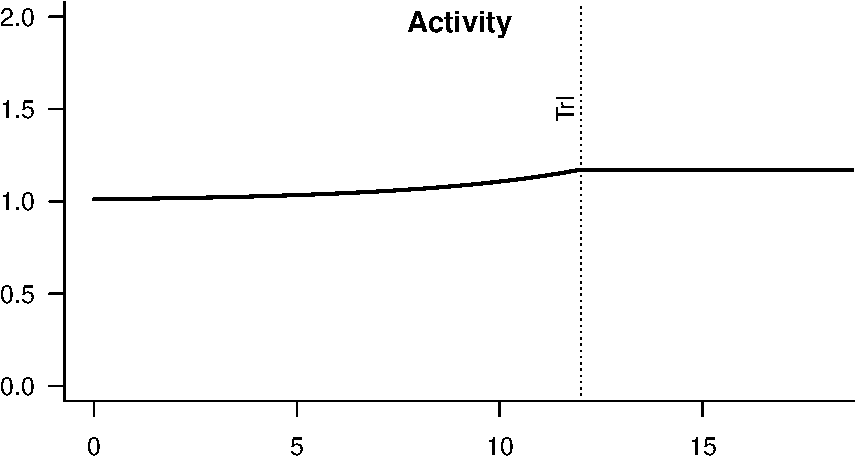
\includegraphics{NRG_summary_files/figure-latex/Part2-3.pdf}

\begin{Shaded}
\begin{Highlighting}[]
  \CommentTok{# now predict waste functions}
    \NormalTok{w_dat<-ebs_data}
    \NormalTok{w_dat$C_in<-}\DecValTok{10}  \CommentTok{# can be grams consumed or joules consumed}
    \KeywordTok{Waste_fun}\NormalTok{(}\DataTypeTok{par=}\NormalTok{PARMS_USE,}\DataTypeTok{data=}\NormalTok{w_dat)}
\end{Highlighting}
\end{Shaded}

\begin{verbatim}
## $F
## [1] 2
## 
## $U
## [1] 0.2656
\end{verbatim}

\begin{Shaded}
\begin{Highlighting}[]
  \CommentTok{# now put it all together for halibut}
  
    \NormalTok{tt<-}\KeywordTok{bioE}\NormalTok{(}\DataTypeTok{par=}\NormalTok{hal_par,}\DataTypeTok{data=}\NormalTok{ebs_data)}

    \KeywordTok{plot}\NormalTok{(tt[[}\DecValTok{2}\NormalTok{]]$TempC,tt[[}\DecValTok{2}\NormalTok{]]$C_ggd*}\DecValTok{100}\NormalTok{,}\DataTypeTok{type=}\StringTok{"l"}\NormalTok{,}\DataTypeTok{lwd=}\DecValTok{2}\NormalTok{,}\DataTypeTok{ylim=}\KeywordTok{c}\NormalTok{(-}\DecValTok{1}\NormalTok{,}\DecValTok{5}\NormalTok{),}\DataTypeTok{xlim=}\KeywordTok{c}\NormalTok{(-}\DecValTok{4}\NormalTok{,}\DecValTok{20}\NormalTok{));}\KeywordTok{abline}\NormalTok{(}\DataTypeTok{h=}\DecValTok{0}\NormalTok{,}\DataTypeTok{lty=}\DecValTok{3}\NormalTok{)}
    \KeywordTok{lines}\NormalTok{(tt[[}\DecValTok{2}\NormalTok{]]$TempC,tt[[}\DecValTok{2}\NormalTok{]]$C_ggd*}\DecValTok{100}\NormalTok{-(tt[[}\DecValTok{2}\NormalTok{]]$R_ggd*}\DecValTok{100}\NormalTok{),}\DataTypeTok{type=}\StringTok{"l"}\NormalTok{,}\DataTypeTok{lwd=}\DecValTok{2}\NormalTok{,}\DataTypeTok{col=}\StringTok{"lightblue"}\NormalTok{)}
    \KeywordTok{lines}\NormalTok{(tt[[}\DecValTok{2}\NormalTok{]]$TempC,tt[[}\DecValTok{2}\NormalTok{]]$C_ggd*}\DecValTok{100}\NormalTok{-(tt[[}\DecValTok{2}\NormalTok{]]$R_ggd+tt[[}\DecValTok{2}\NormalTok{]]$SDA_ggd)*}\DecValTok{100}\NormalTok{,}\DataTypeTok{type=}\StringTok{"l"}\NormalTok{,}\DataTypeTok{lwd=}\DecValTok{2}\NormalTok{,}\DataTypeTok{col=}\StringTok{"blue"}\NormalTok{)}
    \KeywordTok{lines}\NormalTok{(tt[[}\DecValTok{2}\NormalTok{]]$TempC,tt[[}\DecValTok{2}\NormalTok{]]$C_ggd*}\DecValTok{100}\NormalTok{-(tt[[}\DecValTok{2}\NormalTok{]]$F_ggd+tt[[}\DecValTok{2}\NormalTok{]]$R_ggd+tt[[}\DecValTok{2}\NormalTok{]]$SDA_ggd)*}\DecValTok{100}\NormalTok{,}\DataTypeTok{type=}\StringTok{"l"}\NormalTok{,}\DataTypeTok{lwd=}\DecValTok{2}\NormalTok{,}\DataTypeTok{col=}\StringTok{"green"}\NormalTok{)}
    \KeywordTok{lines}\NormalTok{(tt[[}\DecValTok{2}\NormalTok{]]$TempC,tt[[}\DecValTok{2}\NormalTok{]]$C_ggd*}\DecValTok{100}\NormalTok{-(tt[[}\DecValTok{2}\NormalTok{]]$U_ggd+tt[[}\DecValTok{2}\NormalTok{]]$F_ggd+tt[[}\DecValTok{2}\NormalTok{]]$R_ggd+tt[[}\DecValTok{2}\NormalTok{]]$SDA_ggd)*}\DecValTok{100}\NormalTok{,}\DataTypeTok{type=}\StringTok{"l"}\NormalTok{,}\DataTypeTok{lwd=}\DecValTok{2}\NormalTok{,}\DataTypeTok{col=}\StringTok{"purple"}\NormalTok{)}
  \CommentTok{# the difference is what is avail for growth:}
    \KeywordTok{lines}\NormalTok{(tt[[}\DecValTok{2}\NormalTok{]]$TempC,tt[[}\DecValTok{2}\NormalTok{]]$G_ggd*}\DecValTok{100}\NormalTok{,}\DataTypeTok{type=}\StringTok{"l"}\NormalTok{,}\DataTypeTok{lwd=}\DecValTok{2}\NormalTok{,}\DataTypeTok{col=}\StringTok{"red"}\NormalTok{,}\DataTypeTok{ylim=}\KeywordTok{c}\NormalTok{(-}\DecValTok{1}\NormalTok{,}\DecValTok{5}\NormalTok{),}\DataTypeTok{xlim=}\KeywordTok{c}\NormalTok{(-}\DecValTok{4}\NormalTok{,}\DecValTok{20}\NormalTok{));}\KeywordTok{abline}\NormalTok{(}\DataTypeTok{h=}\DecValTok{0}\NormalTok{,}\DataTypeTok{lty=}\DecValTok{3}\NormalTok{)}
\end{Highlighting}
\end{Shaded}

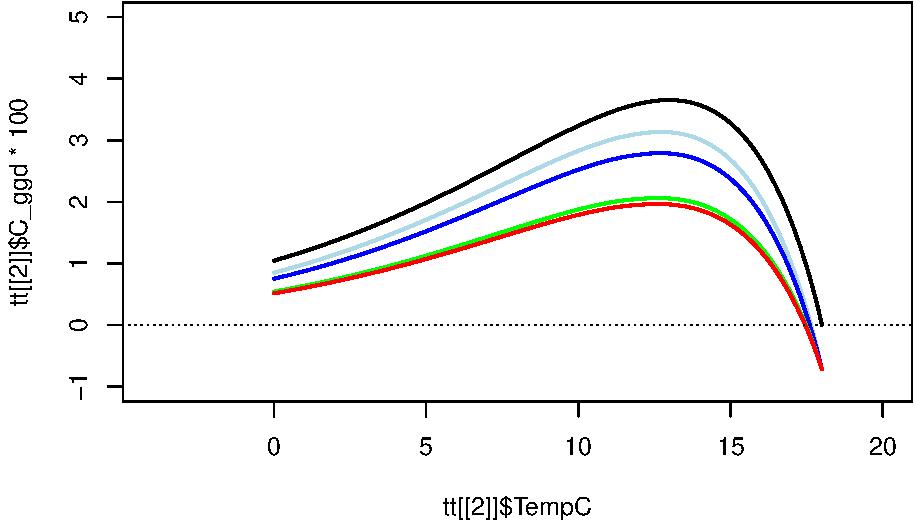
\includegraphics{NRG_summary_files/figure-latex/Part2-4.pdf}

\begin{Shaded}
\begin{Highlighting}[]
    \NormalTok{tt2<-tt}
    \KeywordTok{plot}\NormalTok{(tt2[[}\DecValTok{2}\NormalTok{]]$TempC,tt2[[}\DecValTok{2}\NormalTok{]]$C_ggd*}\DecValTok{100}\NormalTok{,}\DataTypeTok{type=}\StringTok{"l"}\NormalTok{,}\DataTypeTok{lwd=}\DecValTok{2}\NormalTok{,}\DataTypeTok{ylim=}\KeywordTok{c}\NormalTok{(-}\DecValTok{1}\NormalTok{,}\DecValTok{5}\NormalTok{));}\KeywordTok{abline}\NormalTok{(}\DataTypeTok{h=}\DecValTok{0}\NormalTok{,}\DataTypeTok{lty=}\DecValTok{3}\NormalTok{)}
    \KeywordTok{lines}\NormalTok{(tt2[[}\DecValTok{2}\NormalTok{]]$TempC,tt2[[}\DecValTok{2}\NormalTok{]]$G_ggd*}\DecValTok{100}\NormalTok{,}\DataTypeTok{type=}\StringTok{"l"}\NormalTok{,}\DataTypeTok{lwd=}\DecValTok{2}\NormalTok{,}\DataTypeTok{col=}\StringTok{"red"}\NormalTok{)}
    \KeywordTok{lines}\NormalTok{(tt2[[}\DecValTok{2}\NormalTok{]]$TempC,tt2[[}\DecValTok{2}\NormalTok{]]$SDA_ggd*}\DecValTok{100}\NormalTok{,}\DataTypeTok{type=}\StringTok{"l"}\NormalTok{,}\DataTypeTok{lwd=}\DecValTok{2}\NormalTok{,}\DataTypeTok{col=}\StringTok{"lightblue"}\NormalTok{)}
    \KeywordTok{lines}\NormalTok{(tt2[[}\DecValTok{2}\NormalTok{]]$TempC,tt2[[}\DecValTok{2}\NormalTok{]]$R_ggd*}\DecValTok{100}\NormalTok{,}\DataTypeTok{type=}\StringTok{"l"}\NormalTok{,}\DataTypeTok{lwd=}\DecValTok{2}\NormalTok{,}\DataTypeTok{col=}\StringTok{"blue"}\NormalTok{)}
    \KeywordTok{lines}\NormalTok{(tt2[[}\DecValTok{2}\NormalTok{]]$TempC,tt2[[}\DecValTok{2}\NormalTok{]]$U_ggd*}\DecValTok{100}\NormalTok{,}\DataTypeTok{type=}\StringTok{"l"}\NormalTok{,}\DataTypeTok{lwd=}\DecValTok{2}\NormalTok{,}\DataTypeTok{col=}\StringTok{"purple"}\NormalTok{)}
    \KeywordTok{lines}\NormalTok{(tt2[[}\DecValTok{2}\NormalTok{]]$TempC,tt2[[}\DecValTok{2}\NormalTok{]]$F_ggd*}\DecValTok{100}\NormalTok{,}\DataTypeTok{type=}\StringTok{"l"}\NormalTok{,}\DataTypeTok{lwd=}\DecValTok{2}\NormalTok{,}\DataTypeTok{col=}\StringTok{"green"}\NormalTok{)}
\end{Highlighting}
\end{Shaded}

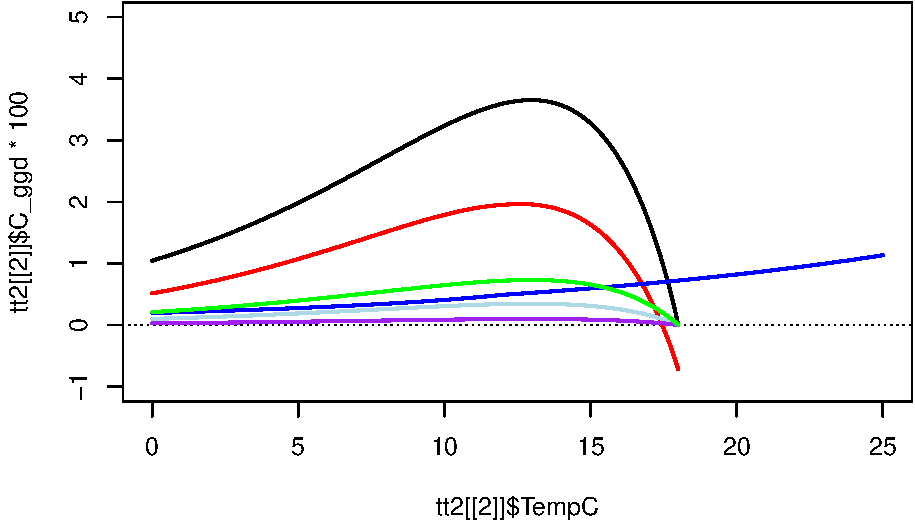
\includegraphics{NRG_summary_files/figure-latex/Part2-5.pdf}

\begin{center}\rule{0.5\linewidth}{\linethickness}\end{center}

\subsection{Part 3: Compare effect of changing prey ED and
quantity}\label{part-3-compare-effect-of-changing-prey-ed-and-quantity}

\begin{Shaded}
\begin{Highlighting}[]
  \CommentTok{# now let's compare to high qual prey}
    \NormalTok{ttH<-}\KeywordTok{bioE}\NormalTok{(}\DataTypeTok{par=}\NormalTok{hal_par,}\DataTypeTok{data=}\NormalTok{ebs_data_highpreyE)}
    \NormalTok{ttL<-}\KeywordTok{bioE}\NormalTok{(}\DataTypeTok{par=}\NormalTok{hal_par,}\DataTypeTok{data=}\NormalTok{ebs_data_lowpreyE)}
  
    \KeywordTok{plot}\NormalTok{(tt[[}\DecValTok{2}\NormalTok{]]$TempC,tt[[}\DecValTok{2}\NormalTok{]]$G_ggd*}\DecValTok{100}\NormalTok{,}\DataTypeTok{type=}\StringTok{"l"}\NormalTok{,}\DataTypeTok{lwd=}\DecValTok{2}\NormalTok{,}\DataTypeTok{ylim=}\KeywordTok{c}\NormalTok{(-}\DecValTok{1}\NormalTok{,}\DecValTok{3}\NormalTok{));}\KeywordTok{abline}\NormalTok{(}\DataTypeTok{h=}\DecValTok{0}\NormalTok{,}\DataTypeTok{lty=}\DecValTok{3}\NormalTok{)}
    \KeywordTok{lines}\NormalTok{(ttH[[}\DecValTok{2}\NormalTok{]]$TempC,ttH[[}\DecValTok{2}\NormalTok{]]$G_ggd*}\DecValTok{100}\NormalTok{,}\DataTypeTok{col=}\StringTok{"red"}\NormalTok{,}\DataTypeTok{lwd=}\DecValTok{2}\NormalTok{)}
    \KeywordTok{lines}\NormalTok{(ttL[[}\DecValTok{2}\NormalTok{]]$TempC,ttL[[}\DecValTok{2}\NormalTok{]]$G_ggd*}\DecValTok{100}\NormalTok{,}\DataTypeTok{col=}\StringTok{"blue"}\NormalTok{,}\DataTypeTok{lwd=}\DecValTok{2}\NormalTok{)}
\end{Highlighting}
\end{Shaded}

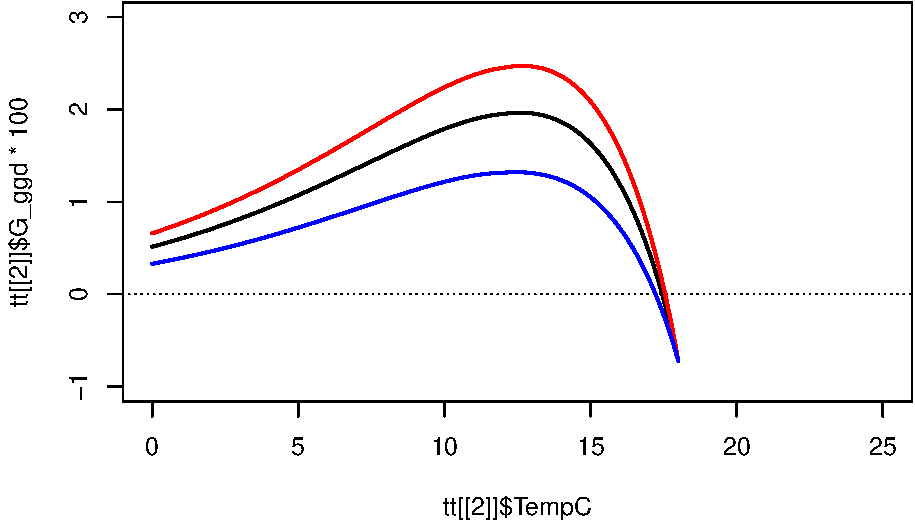
\includegraphics{NRG_summary_files/figure-latex/Part3-1.pdf}

\begin{Shaded}
\begin{Highlighting}[]
  \CommentTok{# now let's compare to lower foraging rate (e.g., less prey)}
    \NormalTok{RFR2<-}\FloatTok{0.4}
    \NormalTok{hal_par2<-hal_par; hal_par2$RFR<-RFR2}
    \NormalTok{ttH04<-}\KeywordTok{bioE}\NormalTok{(}\DataTypeTok{par=}\NormalTok{hal_par2,}\DataTypeTok{data=}\NormalTok{ebs_data_highpreyE)}
    \NormalTok{ttL04<-}\KeywordTok{bioE}\NormalTok{(}\DataTypeTok{par=}\NormalTok{hal_par2,}\DataTypeTok{data=}\NormalTok{ebs_data_lowpreyE)}
    \KeywordTok{par}\NormalTok{(}\DataTypeTok{mfrow=}\KeywordTok{c}\NormalTok{(}\DecValTok{2}\NormalTok{,}\DecValTok{1}\NormalTok{))}
    \KeywordTok{plot}\NormalTok{(tt[[}\DecValTok{2}\NormalTok{]]$TempC,tt[[}\DecValTok{2}\NormalTok{]]$G_ggd*}\DecValTok{100}\NormalTok{,}\DataTypeTok{type=}\StringTok{"l"}\NormalTok{,}\DataTypeTok{lwd=}\DecValTok{2}\NormalTok{,}\DataTypeTok{ylim=}\KeywordTok{c}\NormalTok{(-}\DecValTok{1}\NormalTok{,}\DecValTok{3}\NormalTok{),}\DataTypeTok{ylab=}\StringTok{"Growth (%BW d-1)"}\NormalTok{,}\DataTypeTok{xlab=}\StringTok{""}\NormalTok{);}\KeywordTok{abline}\NormalTok{(}\DataTypeTok{h=}\DecValTok{0}\NormalTok{,}\DataTypeTok{lty=}\DecValTok{3}\NormalTok{)}
    \KeywordTok{lines}\NormalTok{(ttH[[}\DecValTok{2}\NormalTok{]]$TempC,ttH[[}\DecValTok{2}\NormalTok{]]$G_ggd*}\DecValTok{100}\NormalTok{,}\DataTypeTok{col=}\StringTok{"red"}\NormalTok{,}\DataTypeTok{lwd=}\DecValTok{2}\NormalTok{)}
    \KeywordTok{lines}\NormalTok{(ttH04[[}\DecValTok{2}\NormalTok{]]$TempC,ttH04[[}\DecValTok{2}\NormalTok{]]$G_ggd*}\DecValTok{100}\NormalTok{,}\DataTypeTok{col=}\StringTok{"red"}\NormalTok{,}\DataTypeTok{lwd=}\DecValTok{2}\NormalTok{,}\DataTypeTok{lty=}\DecValTok{2}\NormalTok{)}
    \KeywordTok{abline}\NormalTok{(}\DataTypeTok{v=}\NormalTok{ttH04[[}\DecValTok{2}\NormalTok{]]$TempC[ttH04[[}\DecValTok{2}\NormalTok{]]$G_ggd==}\KeywordTok{max}\NormalTok{(ttH04[[}\DecValTok{2}\NormalTok{]]$G_ggd,}\DataTypeTok{na.rm=}\NormalTok{T)],}\DataTypeTok{col=}\StringTok{"red"}\NormalTok{,}\DataTypeTok{lty=}\DecValTok{2}\NormalTok{)}
    \KeywordTok{abline}\NormalTok{(}\DataTypeTok{v=}\NormalTok{ttH[[}\DecValTok{2}\NormalTok{]]$TempC[ttH[[}\DecValTok{2}\NormalTok{]]$G_ggd==}\KeywordTok{max}\NormalTok{(ttH[[}\DecValTok{2}\NormalTok{]]$G_ggd,}\DataTypeTok{na.rm=}\NormalTok{T)],}\DataTypeTok{col=}\StringTok{"red"}\NormalTok{,}\DataTypeTok{lty=}\DecValTok{1}\NormalTok{)}
    \KeywordTok{arrows}\NormalTok{(}\DataTypeTok{x1=}\NormalTok{ttH[[}\DecValTok{2}\NormalTok{]]$TempC[ttH[[}\DecValTok{2}\NormalTok{]]$G_ggd==}\KeywordTok{max}\NormalTok{(ttH[[}\DecValTok{2}\NormalTok{]]$G_ggd,}\DataTypeTok{na.rm=}\NormalTok{T)],}\DataTypeTok{x0=}\DecValTok{20}\NormalTok{,}\DataTypeTok{y1=}\DecValTok{3}\NormalTok{,}\DataTypeTok{y0=}\DecValTok{2}\NormalTok{,}\DataTypeTok{col=}\StringTok{"red"}\NormalTok{,}\DataTypeTok{length =} \FloatTok{0.1}\NormalTok{)}
    \KeywordTok{arrows}\NormalTok{(}\DataTypeTok{x1=}\NormalTok{ttH04[[}\DecValTok{2}\NormalTok{]]$TempC[ttH04[[}\DecValTok{2}\NormalTok{]]$G_ggd==}\KeywordTok{max}\NormalTok{(ttH04[[}\DecValTok{2}\NormalTok{]]$G_ggd,}\DataTypeTok{na.rm=}\NormalTok{T)],}\DataTypeTok{x0=}\DecValTok{20}\NormalTok{,}\DataTypeTok{y1=}\DecValTok{1}\NormalTok{,}\DataTypeTok{y0=}\FloatTok{1.5}\NormalTok{,}\DataTypeTok{col=}\StringTok{"red"}\NormalTok{,}\DataTypeTok{length =} \FloatTok{0.1}\NormalTok{)}
    \KeywordTok{text}\NormalTok{(}\DecValTok{20}\NormalTok{,}\FloatTok{1.5}\NormalTok{, }\KeywordTok{paste0}\NormalTok{(}\StringTok{"max G; RFR="}\NormalTok{,RFR2),}\DataTypeTok{pos=}\DecValTok{4}\NormalTok{,}\DataTypeTok{cex=}\NormalTok{.}\DecValTok{8}\NormalTok{);  }\KeywordTok{text}\NormalTok{(}\DecValTok{20}\NormalTok{,}\DecValTok{2}\NormalTok{, }\StringTok{"max G; RFR=1.0"}\NormalTok{,}\DataTypeTok{pos=}\DecValTok{4}\NormalTok{,}\DataTypeTok{cex=}\NormalTok{.}\DecValTok{8}\NormalTok{)}
    \KeywordTok{mtext}\NormalTok{(}\StringTok{"high prey ED"}\NormalTok{,}\DataTypeTok{side=}\DecValTok{3}\NormalTok{,}\DataTypeTok{adj=}\NormalTok{.}\DecValTok{025}\NormalTok{,}\DataTypeTok{line=}\NormalTok{-}\FloatTok{1.5}\NormalTok{)}
    
    \KeywordTok{plot}\NormalTok{(tt[[}\DecValTok{2}\NormalTok{]]$TempC,tt[[}\DecValTok{2}\NormalTok{]]$G_ggd*}\DecValTok{100}\NormalTok{,}\DataTypeTok{type=}\StringTok{"l"}\NormalTok{,}\DataTypeTok{lwd=}\DecValTok{2}\NormalTok{,}\DataTypeTok{ylim=}\KeywordTok{c}\NormalTok{(-}\DecValTok{1}\NormalTok{,}\DecValTok{3}\NormalTok{),}\DataTypeTok{ylab=}\StringTok{"Growth (%BW d-1)"}\NormalTok{,}\DataTypeTok{xlab=}\StringTok{"Temp (oC)"}\NormalTok{);}\KeywordTok{abline}\NormalTok{(}\DataTypeTok{h=}\DecValTok{0}\NormalTok{,}\DataTypeTok{lty=}\DecValTok{3}\NormalTok{)}
    \KeywordTok{lines}\NormalTok{(ttL[[}\DecValTok{2}\NormalTok{]]$TempC,ttL[[}\DecValTok{2}\NormalTok{]]$G_ggd*}\DecValTok{100}\NormalTok{,}\DataTypeTok{col=}\StringTok{"blue"}\NormalTok{,}\DataTypeTok{lwd=}\DecValTok{2}\NormalTok{)}
    \KeywordTok{lines}\NormalTok{(ttL04[[}\DecValTok{2}\NormalTok{]]$TempC,ttL04[[}\DecValTok{2}\NormalTok{]]$G_ggd*}\DecValTok{100}\NormalTok{,}\DataTypeTok{col=}\StringTok{"blue"}\NormalTok{,}\DataTypeTok{lwd=}\DecValTok{2}\NormalTok{,}\DataTypeTok{lty=}\DecValTok{2}\NormalTok{)}
    \KeywordTok{abline}\NormalTok{(}\DataTypeTok{v=}\NormalTok{ttL04[[}\DecValTok{2}\NormalTok{]]$TempC[ttL04[[}\DecValTok{2}\NormalTok{]]$G_ggd==}\KeywordTok{max}\NormalTok{(ttL04[[}\DecValTok{2}\NormalTok{]]$G_ggd,}\DataTypeTok{na.rm=}\NormalTok{T)],}\DataTypeTok{col=}\StringTok{"blue"}\NormalTok{,}\DataTypeTok{lty=}\DecValTok{2}\NormalTok{)}
    \KeywordTok{abline}\NormalTok{(}\DataTypeTok{v=}\NormalTok{ttL[[}\DecValTok{2}\NormalTok{]]$TempC[ttL[[}\DecValTok{2}\NormalTok{]]$G_ggd==}\KeywordTok{max}\NormalTok{(ttL[[}\DecValTok{2}\NormalTok{]]$G_ggd,}\DataTypeTok{na.rm=}\NormalTok{T)],}\DataTypeTok{col=}\StringTok{"blue"}\NormalTok{,}\DataTypeTok{lty=}\DecValTok{1}\NormalTok{)}
    \KeywordTok{arrows}\NormalTok{(}\DataTypeTok{x1=}\NormalTok{ttL[[}\DecValTok{2}\NormalTok{]]$TempC[ttL[[}\DecValTok{2}\NormalTok{]]$G_ggd==}\KeywordTok{max}\NormalTok{(ttL[[}\DecValTok{2}\NormalTok{]]$G_ggd,}\DataTypeTok{na.rm=}\NormalTok{T)],}\DataTypeTok{x0=}\DecValTok{20}\NormalTok{,}\DataTypeTok{y1=}\FloatTok{2.75}\NormalTok{,}\DataTypeTok{y0=}\DecValTok{2}\NormalTok{,}\DataTypeTok{col=}\StringTok{"blue"}\NormalTok{,}\DataTypeTok{length =} \FloatTok{0.1}\NormalTok{)}
    \KeywordTok{arrows}\NormalTok{(}\DataTypeTok{x1=}\NormalTok{ttL04[[}\DecValTok{2}\NormalTok{]]$TempC[ttL04[[}\DecValTok{2}\NormalTok{]]$G_ggd==}\KeywordTok{max}\NormalTok{(ttL04[[}\DecValTok{2}\NormalTok{]]$G_ggd,}\DataTypeTok{na.rm=}\NormalTok{T)],}\DataTypeTok{x0=}\DecValTok{20}\NormalTok{,}\DataTypeTok{y1=}\DecValTok{1}\NormalTok{,}\DataTypeTok{y0=}\FloatTok{1.5}\NormalTok{,}\DataTypeTok{col=}\StringTok{"blue"}\NormalTok{,}\DataTypeTok{length =} \FloatTok{0.1}\NormalTok{)}
    \KeywordTok{text}\NormalTok{(}\DecValTok{20}\NormalTok{,}\FloatTok{1.5}\NormalTok{, }\KeywordTok{paste0}\NormalTok{(}\StringTok{"max G; RFR="}\NormalTok{,RFR2),}\DataTypeTok{pos=}\DecValTok{4}\NormalTok{,}\DataTypeTok{cex=}\NormalTok{.}\DecValTok{8}\NormalTok{);  }\KeywordTok{text}\NormalTok{(}\DecValTok{20}\NormalTok{,}\DecValTok{2}\NormalTok{, }\StringTok{"max G; RFR=1.0"}\NormalTok{,}\DataTypeTok{pos=}\DecValTok{4}\NormalTok{,}\DataTypeTok{cex=}\NormalTok{.}\DecValTok{8}\NormalTok{)}
    \KeywordTok{mtext}\NormalTok{(}\StringTok{"low prey ED"}\NormalTok{,}\DataTypeTok{side=}\DecValTok{3}\NormalTok{,}\DataTypeTok{adj=}\NormalTok{.}\DecValTok{025}\NormalTok{,}\DataTypeTok{line=}\NormalTok{-}\FloatTok{1.5}\NormalTok{)}
\end{Highlighting}
\end{Shaded}

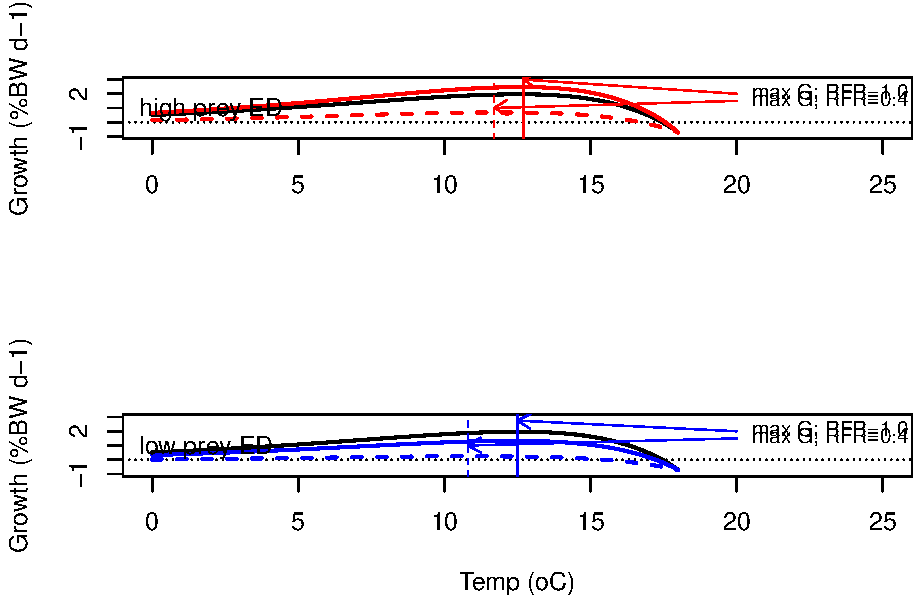
\includegraphics{NRG_summary_files/figure-latex/Part3-2.pdf}

\begin{center}\rule{0.5\linewidth}{\linethickness}\end{center}

\subsection{Part 4: Simulate growth over
time}\label{part-4-simulate-growth-over-time}

\begin{Shaded}
\begin{Highlighting}[]
  \CommentTok{# now let's simulate growth overitme}
    \CommentTok{# load temperature data from A3 area buoy}
    \NormalTok{yr<-}\DecValTok{2005}
    \NormalTok{sub<-all.dat.A3}
    \NormalTok{sub<-sub[sub$Year==yr,]}
    \NormalTok{temp<-}\KeywordTok{tapply}\NormalTok{(sub$Temp,}\KeywordTok{as.character}\NormalTok{(sub$date),mean,}\DataTypeTok{na.rm=}\NormalTok{T)}
    \KeywordTok{head}\NormalTok{(temp)}
\end{Highlighting}
\end{Shaded}

\begin{verbatim}
## 2005-01-01 2005-01-02 2005-01-03 2005-01-04 2005-01-05 2005-01-06 
##   4.821739   5.087500   5.100000   5.195833   5.145833   5.100000
\end{verbatim}

\begin{Shaded}
\begin{Highlighting}[]
    \NormalTok{A3.dat<-}\KeywordTok{data.frame}\NormalTok{(}\DataTypeTok{date=}\KeywordTok{strptime}\NormalTok{(}\KeywordTok{names}\NormalTok{(temp), }\DataTypeTok{format=}\StringTok{"%Y-%m-%d"}\NormalTok{),}\DataTypeTok{Temp=}\NormalTok{temp)}
    \NormalTok{A3.dat<-A3.dat[}\KeywordTok{order}\NormalTok{(A3.dat$date),]}
    \KeywordTok{plot}\NormalTok{(A3.dat,}\DataTypeTok{type=}\StringTok{"l"}\NormalTok{)}
\end{Highlighting}
\end{Shaded}

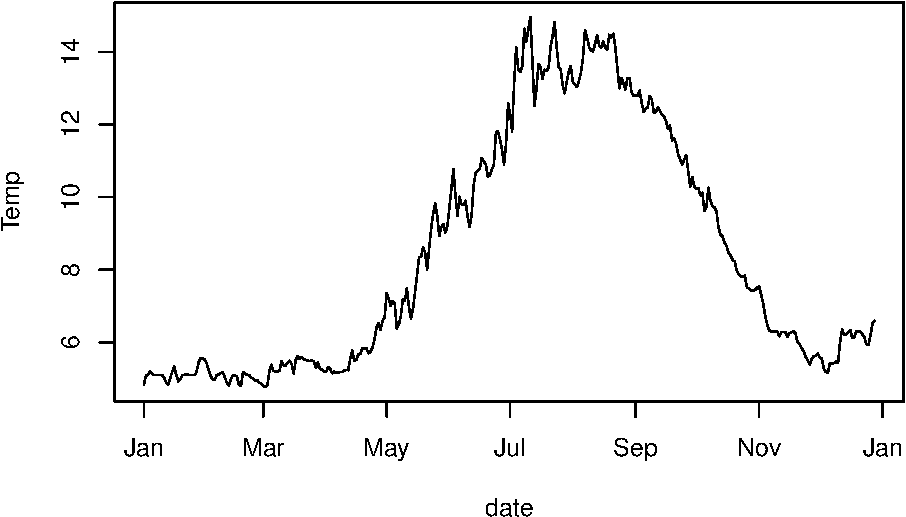
\includegraphics{NRG_summary_files/figure-latex/Part4-1.pdf}

\begin{Shaded}
\begin{Highlighting}[]
    \NormalTok{Tdat<-}\KeywordTok{data.frame}\NormalTok{(}\DataTypeTok{date=}\KeywordTok{seq.Date}\NormalTok{(}\KeywordTok{as.Date}\NormalTok{(}\StringTok{'2005-01-01'}\NormalTok{), }\DataTypeTok{by =} \StringTok{'day'}\NormalTok{, }\DataTypeTok{len =} \DecValTok{365}\NormalTok{),}\DataTypeTok{TempC=}\OtherTok{NA}\NormalTok{)}
    \NormalTok{Tdat$TempC[}\KeywordTok{format}\NormalTok{(Tdat$date,}\StringTok{"%F"}\NormalTok{)%in%}\KeywordTok{format}\NormalTok{(A3.dat$date,}\StringTok{"%F"}\NormalTok{)]<-A3.dat$Temp}
    \NormalTok{cc<-(}\KeywordTok{which}\NormalTok{(}\KeywordTok{is.na}\NormalTok{(Tdat$TempC)))}
    \NormalTok{for(i in }\DecValTok{1}\NormalTok{:}\KeywordTok{length}\NormalTok{(cc)) Tdat$TempC[cc[i]]<-Tdat$TempC[cc[i]-}\DecValTok{1}\NormalTok{]}
    \KeywordTok{plot}\NormalTok{(Tdat,}\DataTypeTok{type=}\StringTok{"l"}\NormalTok{)}
\end{Highlighting}
\end{Shaded}

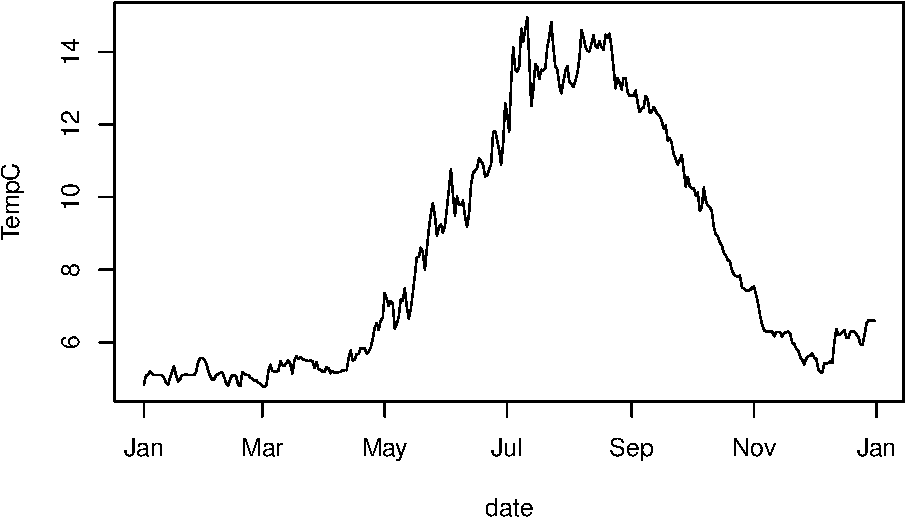
\includegraphics{NRG_summary_files/figure-latex/Part4-2.pdf}

\begin{Shaded}
\begin{Highlighting}[]
    \NormalTok{nd<-}\KeywordTok{dim}\NormalTok{(Tdat)[}\DecValTok{1}\NormalTok{]  }\CommentTok{# number of days}
    \NormalTok{Wstart<-}\DecValTok{200}   \CommentTok{# weight at the start of the simulation}
    \NormalTok{Wobs<-}\KeywordTok{data.frame}\NormalTok{(}\DataTypeTok{day=}\KeywordTok{c}\NormalTok{(}\DecValTok{1}\NormalTok{,}\DecValTok{40}\NormalTok{,}\DecValTok{180}\NormalTok{,}\DecValTok{200}\NormalTok{,}\DecValTok{365}\NormalTok{),}\DataTypeTok{W=}\KeywordTok{c}\NormalTok{(}\DecValTok{200}\NormalTok{,}\DecValTok{220}\NormalTok{,}\DecValTok{350}\NormalTok{,}\DecValTok{400}\NormalTok{,}\DecValTok{500}\NormalTok{)) }\CommentTok{# made up dates and weights}
   
    \NormalTok{par_sim<-hal_par}
    \NormalTok{sim_dat<-ebs_data}
    \NormalTok{sim_dat$Eprey<-}\FloatTok{4598.07}
    \NormalTok{sim_dat$Epred<-}\DecValTok{4800}
    \NormalTok{sim_dat$TempC<-Tdat$TempC}
    \NormalTok{W<-Tdat$TempC*}\DecValTok{0}
    
    \NormalTok{sim_W<-function(}\DataTypeTok{par=}\FloatTok{0.4}\NormalTok{,data,}\DataTypeTok{LL=}\OtherTok{TRUE}\NormalTok{)\{}
      \NormalTok{tmp_par<-data$tmp_par}
      \NormalTok{tmp_par$RFR<-par[}\DecValTok{1}\NormalTok{]}
      \NormalTok{Wtarget<-data$Wtarget}
      \NormalTok{tmp_Tdat<-data$tmp_Tdat}
      \NormalTok{tmp_dat<-data$tmp_dat}
      
      \NormalTok{nd<-}\KeywordTok{dim}\NormalTok{(tmp_Tdat)[}\DecValTok{1}\NormalTok{]}
      \NormalTok{W<-}\KeywordTok{rep}\NormalTok{(}\DecValTok{0}\NormalTok{,nd)}
      \NormalTok{tt<-}\KeywordTok{bioE}\NormalTok{(}\DataTypeTok{par=}\NormalTok{tmp_par,}\DataTypeTok{data=}\NormalTok{tmp_dat)}
      \NormalTok{sim<-}\KeywordTok{data.frame}\NormalTok{(}\KeywordTok{matrix}\NormalTok{(}\DecValTok{0}\NormalTok{,nd,}\KeywordTok{dim}\NormalTok{(tt[[}\DecValTok{2}\NormalTok{]])[}\DecValTok{2}\NormalTok{]))}
      \KeywordTok{colnames}\NormalTok{(sim)<-}\KeywordTok{names}\NormalTok{(tt[[}\DecValTok{2}\NormalTok{]])}
      \NormalTok{sim[}\DecValTok{1}\NormalTok{,]<-tt[[}\DecValTok{2}\NormalTok{]]}
      
      \NormalTok{for(d in }\DecValTok{1}\NormalTok{:nd)\{}
        \CommentTok{# assign weight at the start of day d to that from the previous day}
        \NormalTok{tmp_dat$TempC<-tmp_Tdat$TempC[d]}
        \CommentTok{#if(d==1) tmp_dat$W<-data$Wstart}
        \NormalTok{if(d>}\DecValTok{1}\NormalTok{) tmp_dat$W<-sim$W[d}\DecValTok{-1}\NormalTok{]}
        \NormalTok{tt<-}\KeywordTok{bioE}\NormalTok{(}\DataTypeTok{par=}\NormalTok{tmp_par,}\DataTypeTok{data=}\NormalTok{tmp_dat)}
        \NormalTok{sim[d,]<-tt[[}\DecValTok{2}\NormalTok{]]}
        \NormalTok{sim$W[d]<-sim$W[d]+sim$G_ggd[d]*sim$W[d]  }\CommentTok{# growth in g per d}
      \NormalTok{\}}
      \NormalTok{What<-sim$W[nd]}
      \NormalTok{if(LL)\{}
        \KeywordTok{return}\NormalTok{( ( (Wtarget)-(What) )^}\DecValTok{2} \NormalTok{)}
      \NormalTok{\}else\{}
        \KeywordTok{return}\NormalTok{(sim)}
      \NormalTok{\}}
    \NormalTok{\}}
    
    \NormalTok{sim_dat$W<-Wobs[}\DecValTok{1}\NormalTok{,}\DecValTok{2}\NormalTok{] }\CommentTok{# set W data for the simulation to the first observed weight}
    \NormalTok{subdat<-}\KeywordTok{list}\NormalTok{(}\DataTypeTok{Wtarget=}\NormalTok{Wobs,}\DataTypeTok{tmp_par=}\NormalTok{par_sim,}\DataTypeTok{tmp_Tdat=}\NormalTok{Tdat,}\DataTypeTok{tmp_dat=}\NormalTok{sim_dat) }\CommentTok{# create simulation data file}
    
    \NormalTok{W<-}\KeywordTok{sim_W}\NormalTok{(}\DataTypeTok{par=}\FloatTok{0.4}\NormalTok{,}\DataTypeTok{data=}\NormalTok{subdat,}\DataTypeTok{LL=}\NormalTok{F)$W }\CommentTok{# set Pvalue for whole simulation period, see effect by changing .4 to .6 and rerun}
    \KeywordTok{par}\NormalTok{(}\DataTypeTok{mfrow=}\KeywordTok{c}\NormalTok{(}\DecValTok{1}\NormalTok{,}\DecValTok{1}\NormalTok{))}
    \KeywordTok{plot}\NormalTok{(Wobs,}\DataTypeTok{type=}\StringTok{"b"}\NormalTok{,}\DataTypeTok{ylim=}\KeywordTok{c}\NormalTok{(}\DecValTok{0}\NormalTok{,}\DecValTok{700}\NormalTok{),}\DataTypeTok{main=}\KeywordTok{paste0}\NormalTok{(}\StringTok{"Predicted growth given RFR = "}\NormalTok{,}\FloatTok{0.4}\NormalTok{))}
    \KeywordTok{lines}\NormalTok{(W,}\DataTypeTok{col=}\StringTok{"red"}\NormalTok{)}
\end{Highlighting}
\end{Shaded}

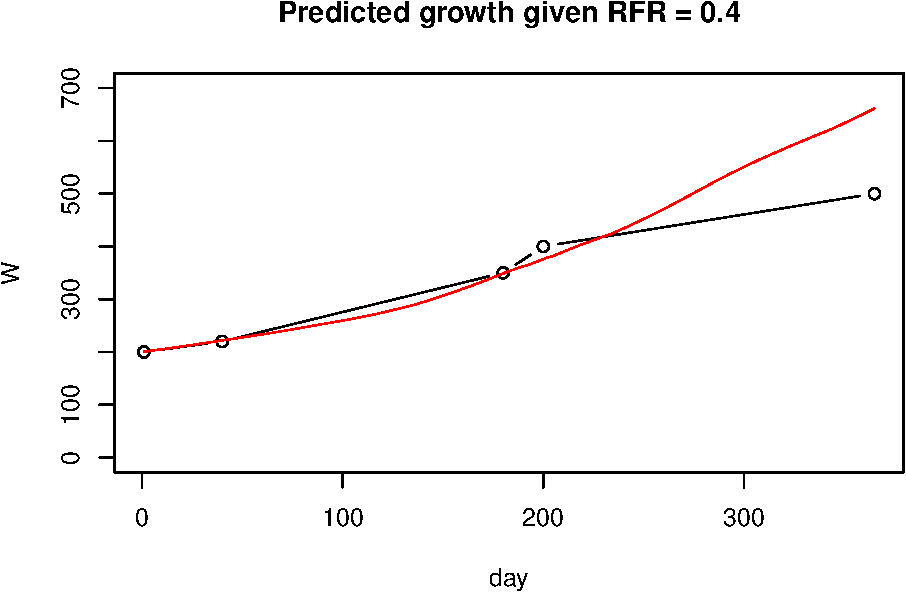
\includegraphics{NRG_summary_files/figure-latex/Part4-3.pdf}

\begin{Shaded}
\begin{Highlighting}[]
    \NormalTok{W<-}\KeywordTok{sim_W}\NormalTok{(}\DataTypeTok{par=}\FloatTok{0.6}\NormalTok{,}\DataTypeTok{data=}\NormalTok{subdat,}\DataTypeTok{LL=}\NormalTok{F)$W }\CommentTok{# set Pvalue for whole simulation period, see effect by changing .4 to .6 and rerun}
    \KeywordTok{par}\NormalTok{(}\DataTypeTok{mfrow=}\KeywordTok{c}\NormalTok{(}\DecValTok{1}\NormalTok{,}\DecValTok{1}\NormalTok{))}
    \KeywordTok{plot}\NormalTok{(Wobs,}\DataTypeTok{type=}\StringTok{"b"}\NormalTok{,}\DataTypeTok{ylim=}\KeywordTok{c}\NormalTok{(}\DecValTok{0}\NormalTok{,}\DecValTok{700}\NormalTok{),}\DataTypeTok{main=}\KeywordTok{paste0}\NormalTok{(}\StringTok{"Predicted growth given RFR = "}\NormalTok{,}\FloatTok{0.6}\NormalTok{))}
    \KeywordTok{lines}\NormalTok{(}\DecValTok{1}\NormalTok{:}\DecValTok{365}\NormalTok{,W,}\DataTypeTok{col=}\StringTok{"red"}\NormalTok{)}
\end{Highlighting}
\end{Shaded}

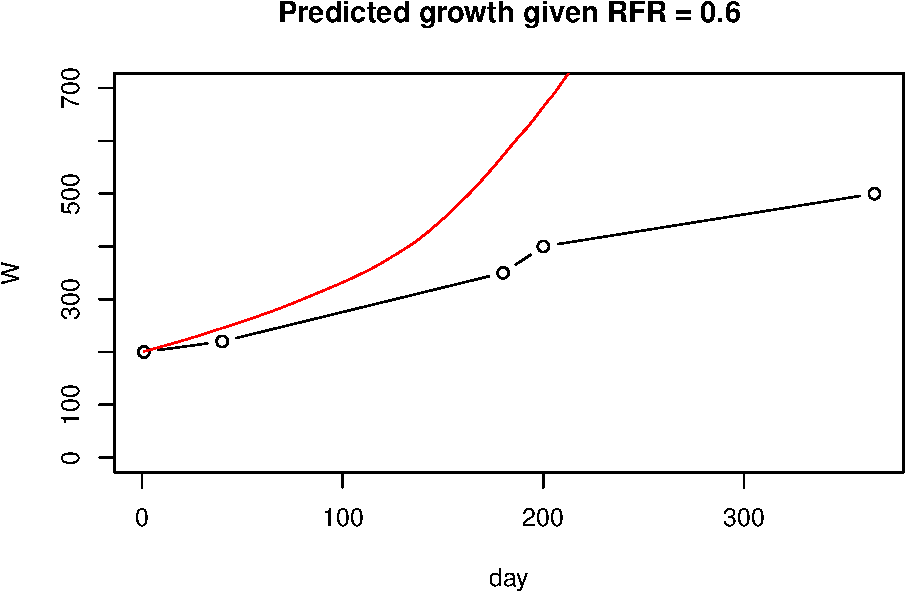
\includegraphics{NRG_summary_files/figure-latex/Part4-4.pdf}

\begin{Shaded}
\begin{Highlighting}[]
  \CommentTok{# now let's fit growth to observed growth overtime by adjusting RFR}
  
    \NormalTok{outdat<-}\KeywordTok{data.frame}\NormalTok{(}\DataTypeTok{day=}\NormalTok{Wobs[,}\DecValTok{1}\NormalTok{],}\DataTypeTok{RFR=}\NormalTok{Wobs[,}\DecValTok{1}\NormalTok{]*}\DecValTok{0}\NormalTok{,}\DataTypeTok{Wobs=}\NormalTok{Wobs[,}\DecValTok{2}\NormalTok{],}\DataTypeTok{What=}\DecValTok{0}\NormalTok{)}
    \NormalTok{sim1<-Tdat}
    \NormalTok{sim1$What<-}\DecValTok{0}
    \NormalTok{sim1$RFR<-}\DecValTok{0}
    \NormalTok{sim1$What[}\DecValTok{1}\NormalTok{]<-Wobs[}\DecValTok{1}\NormalTok{,}\DecValTok{2}\NormalTok{]}
    \NormalTok{nobs<-}\KeywordTok{dim}\NormalTok{(Wobs)[}\DecValTok{1}\NormalTok{]}
    \NormalTok{outdat$What[}\DecValTok{1}\NormalTok{]<-Wobs[}\DecValTok{1}\NormalTok{,}\DecValTok{2}\NormalTok{]}
    \NormalTok{sim_dat$W<-Wobs[}\DecValTok{1}\NormalTok{,}\DecValTok{2}\NormalTok{]}
    
    \NormalTok{for(i in }\DecValTok{2}\NormalTok{:nobs)\{}
      \NormalTok{subTdat<-Tdat[Wobs$day[i}\DecValTok{-1}\NormalTok{]:(Wobs$day[i]-}\DecValTok{1}\NormalTok{),]}
      \NormalTok{sim_dat$W<-outdat$What[i}\DecValTok{-1}\NormalTok{]}
      \NormalTok{subdat<-}\KeywordTok{list}\NormalTok{(}\DataTypeTok{Wtarget=}\NormalTok{Wobs[i,}\DecValTok{2}\NormalTok{],}\DataTypeTok{tmp_par=}\NormalTok{par_sim,}\DataTypeTok{tmp_Tdat=}\NormalTok{subTdat,}\DataTypeTok{tmp_dat=}\NormalTok{sim_dat)}
      \KeywordTok{sim_W}\NormalTok{(}\DataTypeTok{par=}\NormalTok{.}\DecValTok{3}\NormalTok{,}\DataTypeTok{data=}\NormalTok{subdat,}\DataTypeTok{LL=}\OtherTok{TRUE}\NormalTok{)}
      \NormalTok{m<-}\StringTok{ }\KeywordTok{optimize}\NormalTok{(}\DataTypeTok{f=}\NormalTok{sim_W,}\DataTypeTok{lower=}\DecValTok{0}\NormalTok{,}\DataTypeTok{upper=}\DecValTok{10}\NormalTok{,}\DataTypeTok{data=}\NormalTok{subdat,}\DataTypeTok{LL=}\OtherTok{TRUE}\NormalTok{)}
      \NormalTok{outdat$RFR[i]<-(m)[}\DecValTok{1}\NormalTok{]}
      \NormalTok{if(i==}\DecValTok{2}\NormalTok{)  outdat$RFR[i}\DecValTok{-1}\NormalTok{]<-(m)[}\DecValTok{1}\NormalTok{]}
      \NormalTok{sim1[(Wobs$day[i}\DecValTok{-1}\NormalTok{]+}\DecValTok{1}\NormalTok{):(Wobs$day[i]),]$RFR<-(m)[}\DecValTok{1}\NormalTok{]}
      \NormalTok{if(i==}\DecValTok{2}\NormalTok{) tt<-}\KeywordTok{data.frame}\NormalTok{(}\DataTypeTok{day=}\NormalTok{Wobs$day[i}\DecValTok{-1}\NormalTok{]:(Wobs$day[i]-}\DecValTok{1}\NormalTok{),}\KeywordTok{sim_W}\NormalTok{(}\DataTypeTok{par=}\KeywordTok{as.numeric}\NormalTok{(m[}\DecValTok{1}\NormalTok{]),}\DataTypeTok{data=}\NormalTok{subdat,}\DataTypeTok{LL=}\OtherTok{FALSE}\NormalTok{))}
      \NormalTok{if(i>}\DecValTok{2}\NormalTok{) tt<-}\KeywordTok{rbind}\NormalTok{(tt,}\KeywordTok{data.frame}\NormalTok{(}\DataTypeTok{day=}\NormalTok{Wobs$day[i}\DecValTok{-1}\NormalTok{]:(Wobs$day[i]-}\DecValTok{1}\NormalTok{),}\KeywordTok{sim_W}\NormalTok{(}\DataTypeTok{par=}\KeywordTok{as.numeric}\NormalTok{(m[}\DecValTok{1}\NormalTok{]),}\DataTypeTok{data=}\NormalTok{subdat,}\DataTypeTok{LL=}\OtherTok{FALSE}\NormalTok{)))}
      \NormalTok{sim1[(Wobs$day[i}\DecValTok{-1}\NormalTok{]+}\DecValTok{1}\NormalTok{):(Wobs$day[i]),]$What<-tt$W[Wobs$day[i}\DecValTok{-1}\NormalTok{]:(Wobs$day[i]-}\DecValTok{1}\NormalTok{)]}
      \NormalTok{outdat$What[i]<-}\KeywordTok{rev}\NormalTok{(tt$W[Wobs$day[i}\DecValTok{-1}\NormalTok{]:(Wobs$day[i]-}\DecValTok{1}\NormalTok{)])[}\DecValTok{1}\NormalTok{]}
    \NormalTok{\}}
    \NormalTok{sim2<-tt}
    
    \NormalTok{sim_dat$W<-Wobs[}\DecValTok{1}\NormalTok{,}\DecValTok{2}\NormalTok{] }\CommentTok{# set W data for the simulation to the first observed weight}
    \NormalTok{subdat<-}\KeywordTok{list}\NormalTok{(}\DataTypeTok{Wtarget=}\NormalTok{Wobs,}\DataTypeTok{tmp_par=}\NormalTok{par_sim,}\DataTypeTok{tmp_Tdat=}\NormalTok{Tdat,}\DataTypeTok{tmp_dat=}\NormalTok{sim_dat) }\CommentTok{# create simulation data file}
    \KeywordTok{plot}\NormalTok{(Wobs,}\DataTypeTok{type=}\StringTok{"b"}\NormalTok{,}\DataTypeTok{ylim=}\KeywordTok{c}\NormalTok{(}\DecValTok{0}\NormalTok{,}\DecValTok{700}\NormalTok{),}\DataTypeTok{main=}\KeywordTok{paste0}\NormalTok{(}\StringTok{"Predicted growth given RFR = "}\NormalTok{,.}\DecValTok{4}\NormalTok{))}
    \KeywordTok{lines}\NormalTok{(}\DecValTok{1}\NormalTok{:}\DecValTok{365}\NormalTok{,}\KeywordTok{sim_W}\NormalTok{(}\DataTypeTok{par=}\FloatTok{0.4}\NormalTok{,}\DataTypeTok{data=}\NormalTok{subdat,}\DataTypeTok{LL=}\NormalTok{F)$W,}\DataTypeTok{col=}\StringTok{"red"}\NormalTok{)}
    \KeywordTok{lines}\NormalTok{(}\DecValTok{1}\NormalTok{:}\DecValTok{365}\NormalTok{,sim1$What,}\DataTypeTok{col=}\StringTok{"blue"}\NormalTok{,}\DataTypeTok{type=}\StringTok{"l"}\NormalTok{)}
    \KeywordTok{points}\NormalTok{(outdat$day,outdat$What,}\DataTypeTok{pch=}\DecValTok{16}\NormalTok{,}\DataTypeTok{col=}\StringTok{"blue"}\NormalTok{)}
\end{Highlighting}
\end{Shaded}

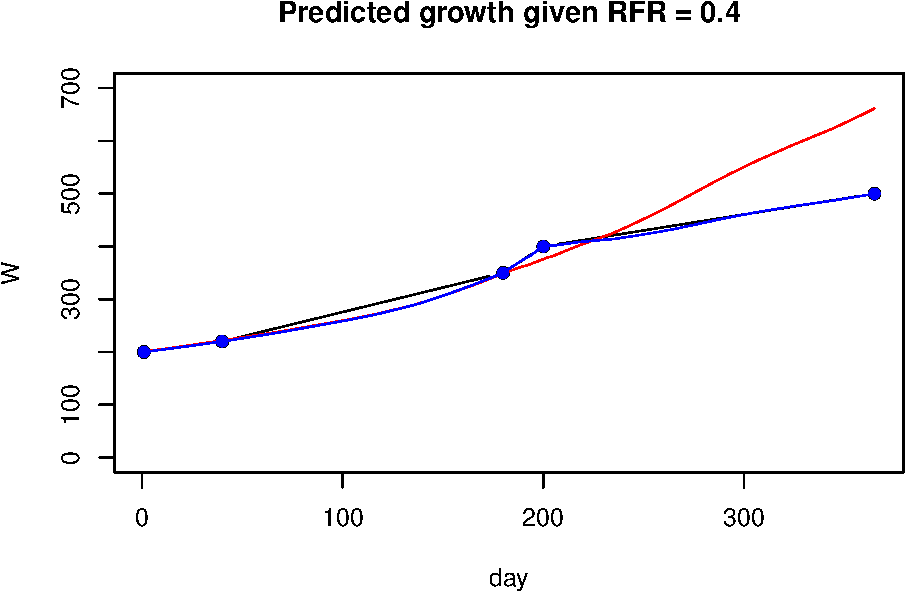
\includegraphics{NRG_summary_files/figure-latex/Part4-5.pdf}

\begin{Shaded}
\begin{Highlighting}[]
    \KeywordTok{plot}\NormalTok{(sim2$day,sim2$fTc,}\DataTypeTok{type=}\StringTok{"l"}\NormalTok{)}
\end{Highlighting}
\end{Shaded}

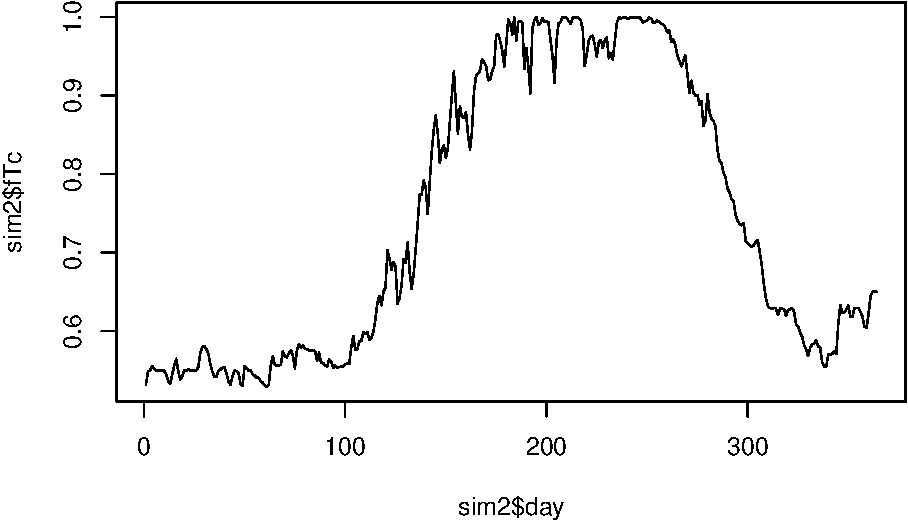
\includegraphics{NRG_summary_files/figure-latex/Part4-6.pdf}

\begin{Shaded}
\begin{Highlighting}[]
    \KeywordTok{plot}\NormalTok{(sim2$day,sim2$RFR,}\DataTypeTok{type=}\StringTok{"l"}\NormalTok{,}\DataTypeTok{ylim=}\KeywordTok{c}\NormalTok{(}\DecValTok{0}\NormalTok{,}\DecValTok{1}\NormalTok{))}
\end{Highlighting}
\end{Shaded}

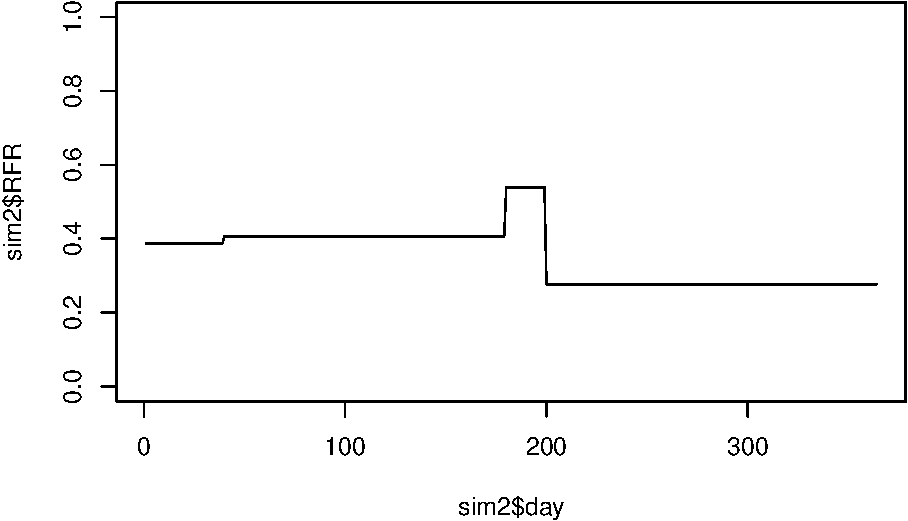
\includegraphics{NRG_summary_files/figure-latex/Part4-7.pdf}

\begin{Shaded}
\begin{Highlighting}[]
    \KeywordTok{plot}\NormalTok{(sim2$day,sim2$G_ggd,}\DataTypeTok{type=}\StringTok{"l"}\NormalTok{)}
\end{Highlighting}
\end{Shaded}

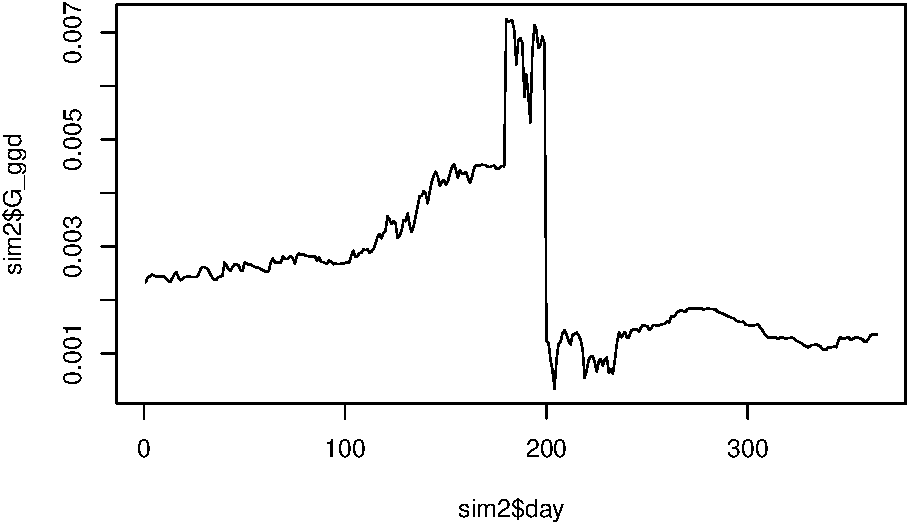
\includegraphics{NRG_summary_files/figure-latex/Part4-8.pdf}

\begin{center}\rule{0.5\linewidth}{\linethickness}\end{center}

\subsection{Part 5: Fit parameters}\label{part-5-fit-parameters}

\begin{Shaded}
\begin{Highlighting}[]
  \CommentTok{# fit pars to lab data:}
      \NormalTok{find_ftcpar<-function(}\DataTypeTok{par=}\KeywordTok{c}\NormalTok{(}\DataTypeTok{logTco=}\KeywordTok{log}\NormalTok{(}\DecValTok{8}\NormalTok{),}\DataTypeTok{logQc=}\KeywordTok{log}\NormalTok{(}\DecValTok{2}\NormalTok{),}
                                  \DataTypeTok{logsigma=}\KeywordTok{log}\NormalTok{(.}\DecValTok{0002}\NormalTok{)),}\DataTypeTok{data=}\KeywordTok{list}\NormalTok{(}\DataTypeTok{c_data=}\NormalTok{c_data,}\DataTypeTok{FTdat=}\NormalTok{FTdat))\{}
        \NormalTok{FTdat<-data$FTdat}
        \NormalTok{c_data<-data$c_data}
        \NormalTok{PARMS_USE$Tco<-}\KeywordTok{exp}\NormalTok{(par[}\DecValTok{1}\NormalTok{])}
        \NormalTok{PARMS_USE$QC<-}\KeywordTok{exp}\NormalTok{(par[}\DecValTok{2}\NormalTok{])}
        \NormalTok{sigma<-}\KeywordTok{exp}\NormalTok{(par[}\DecValTok{3}\NormalTok{])}
        \NormalTok{c_data$TempC<-FTdat$TempC}
        \NormalTok{fThat<-}\KeywordTok{fTC_fun}\NormalTok{(}\DataTypeTok{par=}\NormalTok{PARMS_USE,}\DataTypeTok{data=}\NormalTok{c_data)}
        \NormalTok{LL<-}\KeywordTok{dnorm}\NormalTok{(fThat-FTdat$fTobs,sigma,}\DataTypeTok{log=}\OtherTok{TRUE}\NormalTok{)}
        \NormalTok{LLuse<--}\KeywordTok{sum}\NormalTok{(LL)}
        \NormalTok{if(}\KeywordTok{is.na}\NormalTok{(LLuse))\{LLuse<-}\FloatTok{1e6}\NormalTok{\}    }
        \CommentTok{#if(Tcm>35)\{LLuse<-1e6\} }
        \KeywordTok{return}\NormalTok{(LLuse)}
      \NormalTok{\}}
      \NormalTok{m<-}\KeywordTok{optim}\NormalTok{(}\DataTypeTok{fn=}\NormalTok{find_ftcpar,}\DataTypeTok{par=}\KeywordTok{c}\NormalTok{(}\DataTypeTok{logTco=}\KeywordTok{log}\NormalTok{(}\DecValTok{8}\NormalTok{),}\DataTypeTok{logQc=}\KeywordTok{log}\NormalTok{(}\DecValTok{2}\NormalTok{),}
                \DataTypeTok{logsigma=}\KeywordTok{log}\NormalTok{(.}\DecValTok{0002}\NormalTok{)),}\DataTypeTok{data=}\KeywordTok{list}\NormalTok{(}\DataTypeTok{c_data=}\NormalTok{c_data,}\DataTypeTok{FTdat=}\NormalTok{FTdat),}
                \DataTypeTok{hessian=}\OtherTok{TRUE}\NormalTok{,}\DataTypeTok{control=}\KeywordTok{list}\NormalTok{(}\DataTypeTok{maxit=}\FloatTok{1e6}\NormalTok{))}
      \NormalTok{vc <-}\StringTok{ }\KeywordTok{solve}\NormalTok{(m$hessian)}
      \NormalTok{se<-(}\KeywordTok{sqrt}\NormalTok{(}\KeywordTok{diag}\NormalTok{(vc)))}
      \CommentTok{# not working}
       \CommentTok{#abline(v=exp(m$par[1])+1.95*exp(se[1])); abline(v=exp(m$par[1])-1.95*exp(se[1]))}
      \CommentTok{# p1<-p2<-PARMS_USE}
      \CommentTok{# p1$Tco<-as.numeric(exp(m$par[1]+1*se[1]))}
      \CommentTok{# p1$QC<-as.numeric(exp(m$par[2]+1*se[2]))}
      \CommentTok{# p2$Tco<-as.numeric(exp(m$par[1]-1*se[1]))}
      \CommentTok{# p2$QC<-as.numeric(exp(m$par[2]-1*se[2]))}
      \CommentTok{# lines(ebs_data$TempC,fTC_fun(par=p1,data=c_data))}
      \CommentTok{# lines(ebs_data$TempC,fTC_fun(par=p2,data=c_data))}
      \CommentTok{# }
      
      \CommentTok{# compare values}
      \KeywordTok{round}\NormalTok{(}\KeywordTok{exp}\NormalTok{(m$par),}\DecValTok{3}\NormalTok{)}
\end{Highlighting}
\end{Shaded}

\begin{verbatim}
##   logTco    logQc logsigma 
##   12.970    3.084    0.000
\end{verbatim}

\begin{Shaded}
\begin{Highlighting}[]
      \NormalTok{hal_par$Tco}
\end{Highlighting}
\end{Shaded}

\begin{verbatim}
## [1] 12.9699
\end{verbatim}

\begin{Shaded}
\begin{Highlighting}[]
      \NormalTok{hal_par$QC}
\end{Highlighting}
\end{Shaded}

\begin{verbatim}
## [1] 3.084
\end{verbatim}


\end{document}
